\chapter{Banco de Dados - SGBDs x NoSQL}
\thispagestyle{empty}
Este capitulo procura estabelecer além de uma breve introdução terminológica, um comparativo entre banco de dados relacionais e os NoSQL.

\section{Breve Histórico}
Atualmente o mundo enfrenta uma quantidade siguinificativa, mediante a demanda de dados trafegados simultaneamente pela rede. Desde o surgimento do modelo
relacional de armazenamento de dados por \cite{CODD}, este tem sido abrangentemente utilizado ao redor do mundo para diversas finalidades. Esse sistema de 
gerenciamento de banco dados \textbf{mundialmente} conhecido como SGBDs, tais como Mysql, PostgreSQL, Oracle, SQLServer entre outros foram sendo utilizados ao 
percurso de muitos anos, sendo estes adotados como padrão por muitas empresas desde comuns até desenvolvedoras de \textbf{software}, atendendo comletamente ao
propósito de cada uma com suas diferentes situações e aplicações, contudo com o avanço das tecnologias empregadas no ramo do desenvolvimento de sistemsas web 
no \textit{século XXI}, com o grande aumento da demanda de dados e com o advento do surgimento das redes sociais, grandes portais com número, intermitente de
informações a todo momento, sites de compra coletiva entre outros tipos de sistemas, a arquitetura dos \textbf{SGBDs} começou a ser questionada por apresentar 
certas limitações quanto a escalabilidade e performance. A escalabilidade de um SGBD está relacionada à capacidade de um software crescer de tal forma, rápida
e intuitiva e eficiente, que possa atender a uma demanda cada vez maior de dados. A performance do software que faz uso de um SGBDs, por sua vez, faz referência
à estimativa do tempo de resposta das requisições efetuadas pelo usuário que faz uso de determinado sistema.

Tendo em vista, o surgimento dessas novas aplicações, fez com que a indústria de de desenvolvimento de software apresentasse novas idéias expecificas para estas
duas situações concistentes e existentes devido às limitações dos sistemas de armazenamento de dados relacionais. As novas aplicações web exploram conteúdo em 
abrangencia na Web 2.0 e diante dos problemas encontrados, foram desenvolvidas novas soluções proprietárias, que diferem do paradigma relacional, 
as quais foram todas reunidas sob a nomenclatura \textit{NoSQL (Not Only SQL)}.\cite{CUNHA}.

\section{SGBDs Relacionais}
Existe uma ampla diferença entre Dados, Informação e Conhecimento.
\begin{itemize}
  \item{ \textbf{ Dado: } Qualquer fato, instrução formalizada para uso da comunicação, um código para uma obra-prima de objetos, ou seja é a informação não tratada.
  
    \centering{ \textit{"Dados são itens referentes a uma descrição primária de objetos, eventos, atividades e transações 
    que são gravados, classificados e armazenados, mas não chegam a ser organizados de forma a transmitir 
    algum significado específico."}\cite{MCLEAN_WETHERBE}.}
  }

  \item{ \textbf{ Informação: } É a coleção de tudo aquilo que faz sentido e possui valor constitucional e siguinificante aquelas às quais pode se tirar algum proveito para determinado propósito.
  
    \centering{ \textit{"Informação é todo conjunto de dados organizados de forma a terem sentido e valor para seu destinatário. 
      Este interpreta o significado, tira conclusões e faz deduções a partir deles"}\cite{MCLEAN_WETHERBE}. } 
  }
  
  \item{ \textbf{ Conhecimento: } Segundo \cite{MCLEAN_WETHERBE}, assim como conhecimentto É a coleção de tudo aquilo que faz sentido e possui valor constitucional e siguinificante 
    aquelas às quais pode se tirar algum proveito para determinado propósito, conhecimento é a junção de todos os dados e informações processados afim de transmitir
    a compreensão, experiência, aprendizado acumulativo e alguma técnica, quando aplicada a determinada situação ou atividade que dependa de tal conhecimento. 
  }
\end{itemize}

Em uma base de dados todo e qualquer dado obtido através de um sistema é armazenado e a partir dessa informação contida pode-se obter conhecimento através do processamento
dessa coleção de dados e informação. Uma das grandes e principais características do modelo de dados relacionais são as restrições de integridade:

O termo integridade em banco de dados é amplamente utilizado com o seguinte siguinificado: (presisão, correção e validação) e com isso vem o grande problema de muitos sistemas, 
assegurar que os dados contidos nas tabelas se mantenham precisos, validos e corretos. Visto que se o objetivo do controle de acesso à base de dados é o de evitar que pessoas e/ou programas 
não autorizados leiam e/ou atualizem ou até mesmo realizem exclusões na base de dados, então é objetivo dos mecanismos que zelam pela integridade semântica do BD garantir que somente 
atualizações permitidas sejam executadas na base de dados.

\section{Teorema de CAP}
A famosa palestra do Drº Erich Brewer professor da Universidade da Califórnia apresentada no simpósio sobre princípios da computação distribuída \textbf{ (Principles of Distributed Computing - PODC) } 
apresentada em 2000, introduz a afirmativa do teorema e explica que qualquer em sistema distribuído estável é preciso escolher entre consistência forte (C – Consistency), alta disponibilidade (A – availability) e tolerância a particionamento dos dados na rede(P – Network Partition Tolerance)
Essa afirmação mais tarde no ano de 2002 foi comprovada por \textbf{ Seth Gilbert e Nancy Lynch } se tornando conhecida como teorema de Brewer ou teorema de CAP. \cite{BREWER}.

\begin{figure}[ht]
    \centering
    \scalebox{0.4}{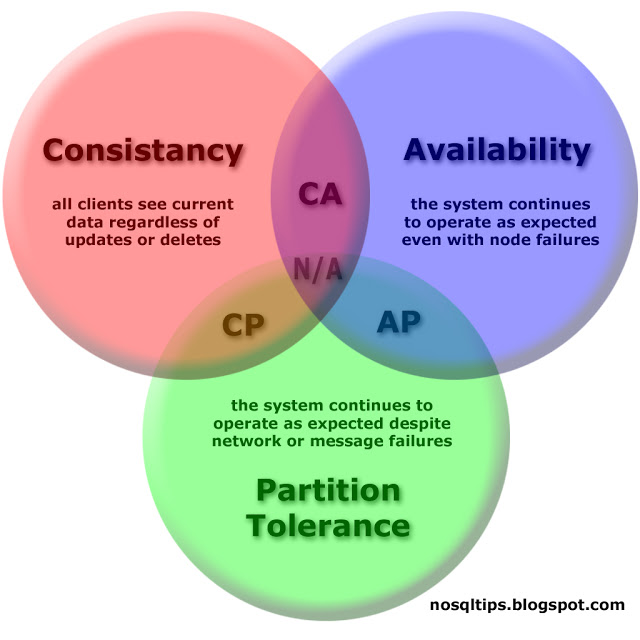
\includegraphics{figuras/CAP_Diagram}}
    \caption{Diagrama do Teorema de CAP(Brewer)}
    \label{submeter}
\end{figure}


\subsection{ C – Consistência }
É considerada como a característica que transcreve as duas condicionais de um sistema, como o sistema fica consistente após e
uma operação e se ele fica consistente. Uma base de dados consistênte distribuida é dita como fortemente consistente ou 
como tendo fraca consistência. Os sistemas com uma forte consistência, implementam as características ACID 
(Atomicidade, Consistência, Isolamento e Durabilidade), sendo estas implementadas na maior parte das bases de dados relacionais. 
Na outra extremidade, de fraca consistência, temos as bases de dados BASE (Basic Availability, Soft-State, Eventual 
Consistency).

\subsection{ A – Disponibilidade }
A disponibilidade que, segundo \cite{BROWNE}, deve garantir que um sistema esteja sempre fornecendo acesso e funcionalidades a seus usuários, 
é uma das propriedades mais importantes e indispensável para sistemas de empresas, sejam eles baseados em Web ou não mas  que precisam disponibilizar
seus serviços continuamente, por exemplo, empresas como a Google ou a Microsoft. Entretanto inevitáveis falhas podem ocorrer, e é nesse momento em que 
alguma contingência (backups automáticos e alguma redundância) deve ocorrer para minimizar o impacto ao usuário.

\subsection{ P – Tolerância ao Particionamento }

\section{NoSQL}

\section{Comparativo entre SGBDS Relacionais e Não Relacionais}
